\section{Introduction}

A Geometric Transformation is any function \[f:\mathbb{R}^m\to\mathbb{R}^n\] In the case of image processing, we are concerned with functions from $\mathbb{R}^2$ to $\mathbb{R}^2$.

\href{https://github.com/TetroVolt/DIP-Project}{Our application} allows the user to apply various geometric transformations to images. This report describes these transformations and details some observations made during development and the ways these transformations can be used to determine properties of an image. 

All images in this report are transformations applied to the following image of Lenna.

\begin{figure}[H]
    \centering
    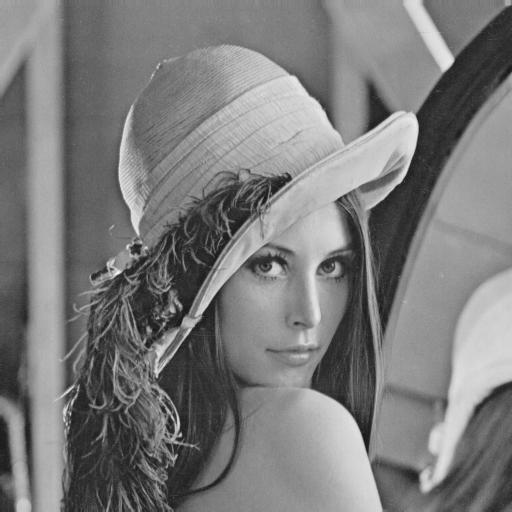
\includegraphics[scale=0.5]{images/lenna-grey.jpg}
    \caption{Lenna}
    \label{fig:lenna-original}
\end{figure}